\section{Results}

\subsection{Summary of Data and Model Selection}

The final analysis comprised 1,894 analyzable observation pairs collected across 115 unique deployment-day combinations from two overwintering sites during the 2023-2024 season. These observations captured monarch abundance changes at 30-minute intervals under varying environmental conditions. We employed a Generalized Additive Mixed Model (GAMM) framework to test 47 candidate models, with model selection performed using an information-theoretic approach based on the Akaike Information Criterion (AIC).

The best-fit model (M23) included smooth terms for previous butterfly count, average temperature, butterflies in direct sunlight, and time within day, achieving an AIC value of 8081.848 (Table \ref{tab:model_selection}). This model carried 88\% of the support among all candidate models (AIC weight = 0.88), with the next-best model (M22) showing substantially less support (ΔAIC = 4.796). Notably, model M24, which included maximum wind gust as an additional predictor, performed worse than M23 (ΔAIC = 6.2), and wind variables appeared in none of the top-performing models.

\begin{table}[htbp]
\centering
\caption{Model selection results showing the top five candidate models ranked by AIC. Model terms are shown with their respective AIC values, ΔAIC relative to the best model, and AIC weights. Wind p-values are shown where applicable; NA indicates the model did not include wind variables.}
\label{tab:model_selection}
\begin{tabular}{lllrrr}
\hline
Model & Terms & AIC & ΔAIC & Weight & Wind p \\
\hline
M23 & Lagged butterflies, Temperature, & 8081.8 & 0.0 & 0.880 & NA \\
    & Sun exposure, Time of day & & & & \\
M22 & Lagged butterflies, Temperature (linear), & 8086.6 & 4.8 & 0.080 & NA \\
    & Sun exposure, Time of day & & & & \\
M24 & Lagged butterflies, Max gust, Temperature, & 8088.0 & 6.2 & 0.040 & 0.218 \\
    & Sun exposure, Time of day & & & & \\
M47 & Temperature, Sun exposure, & 8101.3 & 19.4 & <0.001 & NA \\
    & Time of day & & & & \\
M17 & Lagged butterflies, Temperature, & 8105.9 & 24.0 & <0.001 & NA \\
    & Sun exposure & & & & \\
\hline
\end{tabular}
\end{table}

\subsection{Analysis of the Best-Fit Model}

The best-fit model (M23) explained a modest but significant portion of variance in monarch abundance changes (adjusted R² = 0.057). The model formula was:

\begin{equation}
\text{butterfly\_difference\_cbrt} \sim s(\text{total\_butterflies\_t\_lag}) + s(\text{temperature\_avg}) + 
\end{equation}
\begin{equation*}
s(\text{butterflies\_direct\_sun\_t\_lag}) + s(\text{time\_within\_day\_t})
\end{equation*}

where $s()$ denotes smooth terms estimated using penalized regression splines. All four smooth terms showed significant effects on monarch abundance changes (Table \ref{tab:smooth_terms}).

\begin{table}[htbp]
\centering
\caption{Summary of smooth terms in the best-fit model (M23). EDF represents effective degrees of freedom, indicating the complexity of each smooth relationship.}
\label{tab:smooth_terms}
\begin{tabular}{lrrrr}
\hline
Term & EDF & Ref. df & F-value & p-value \\
\hline
Lagged roost size & 2.62 & 2.62 & 12.02 & 8.26e-07 \\
Average temperature & 3.93 & 3.93 & 3.23 & 0.028 \\
Direct sun exposure & 1.53 & 1.53 & 19.36 & 1.22e-05 \\
Time within day & 4.90 & 4.90 & 8.90 & <2e-16 \\
\hline
\end{tabular}
\end{table}

The previous butterfly count showed a significant non-linear negative relationship with abundance change (effective degrees of freedom [EDF] = 2.62, F = 12.02, p < 0.001). As the initial roost size increased, the change in abundance became increasingly negative, indicating proportionally greater departures from larger aggregations (Figure \ref{fig:effect_roost_size}). Average temperature exhibited a complex non-linear relationship (EDF = 3.93, F = 3.23, p = 0.028), with positive effects on monarch movement peaking at approximately 20°C before declining at higher temperatures (Figure \ref{fig:effect_temperature}).

\begin{figure}[htbp]
\centering
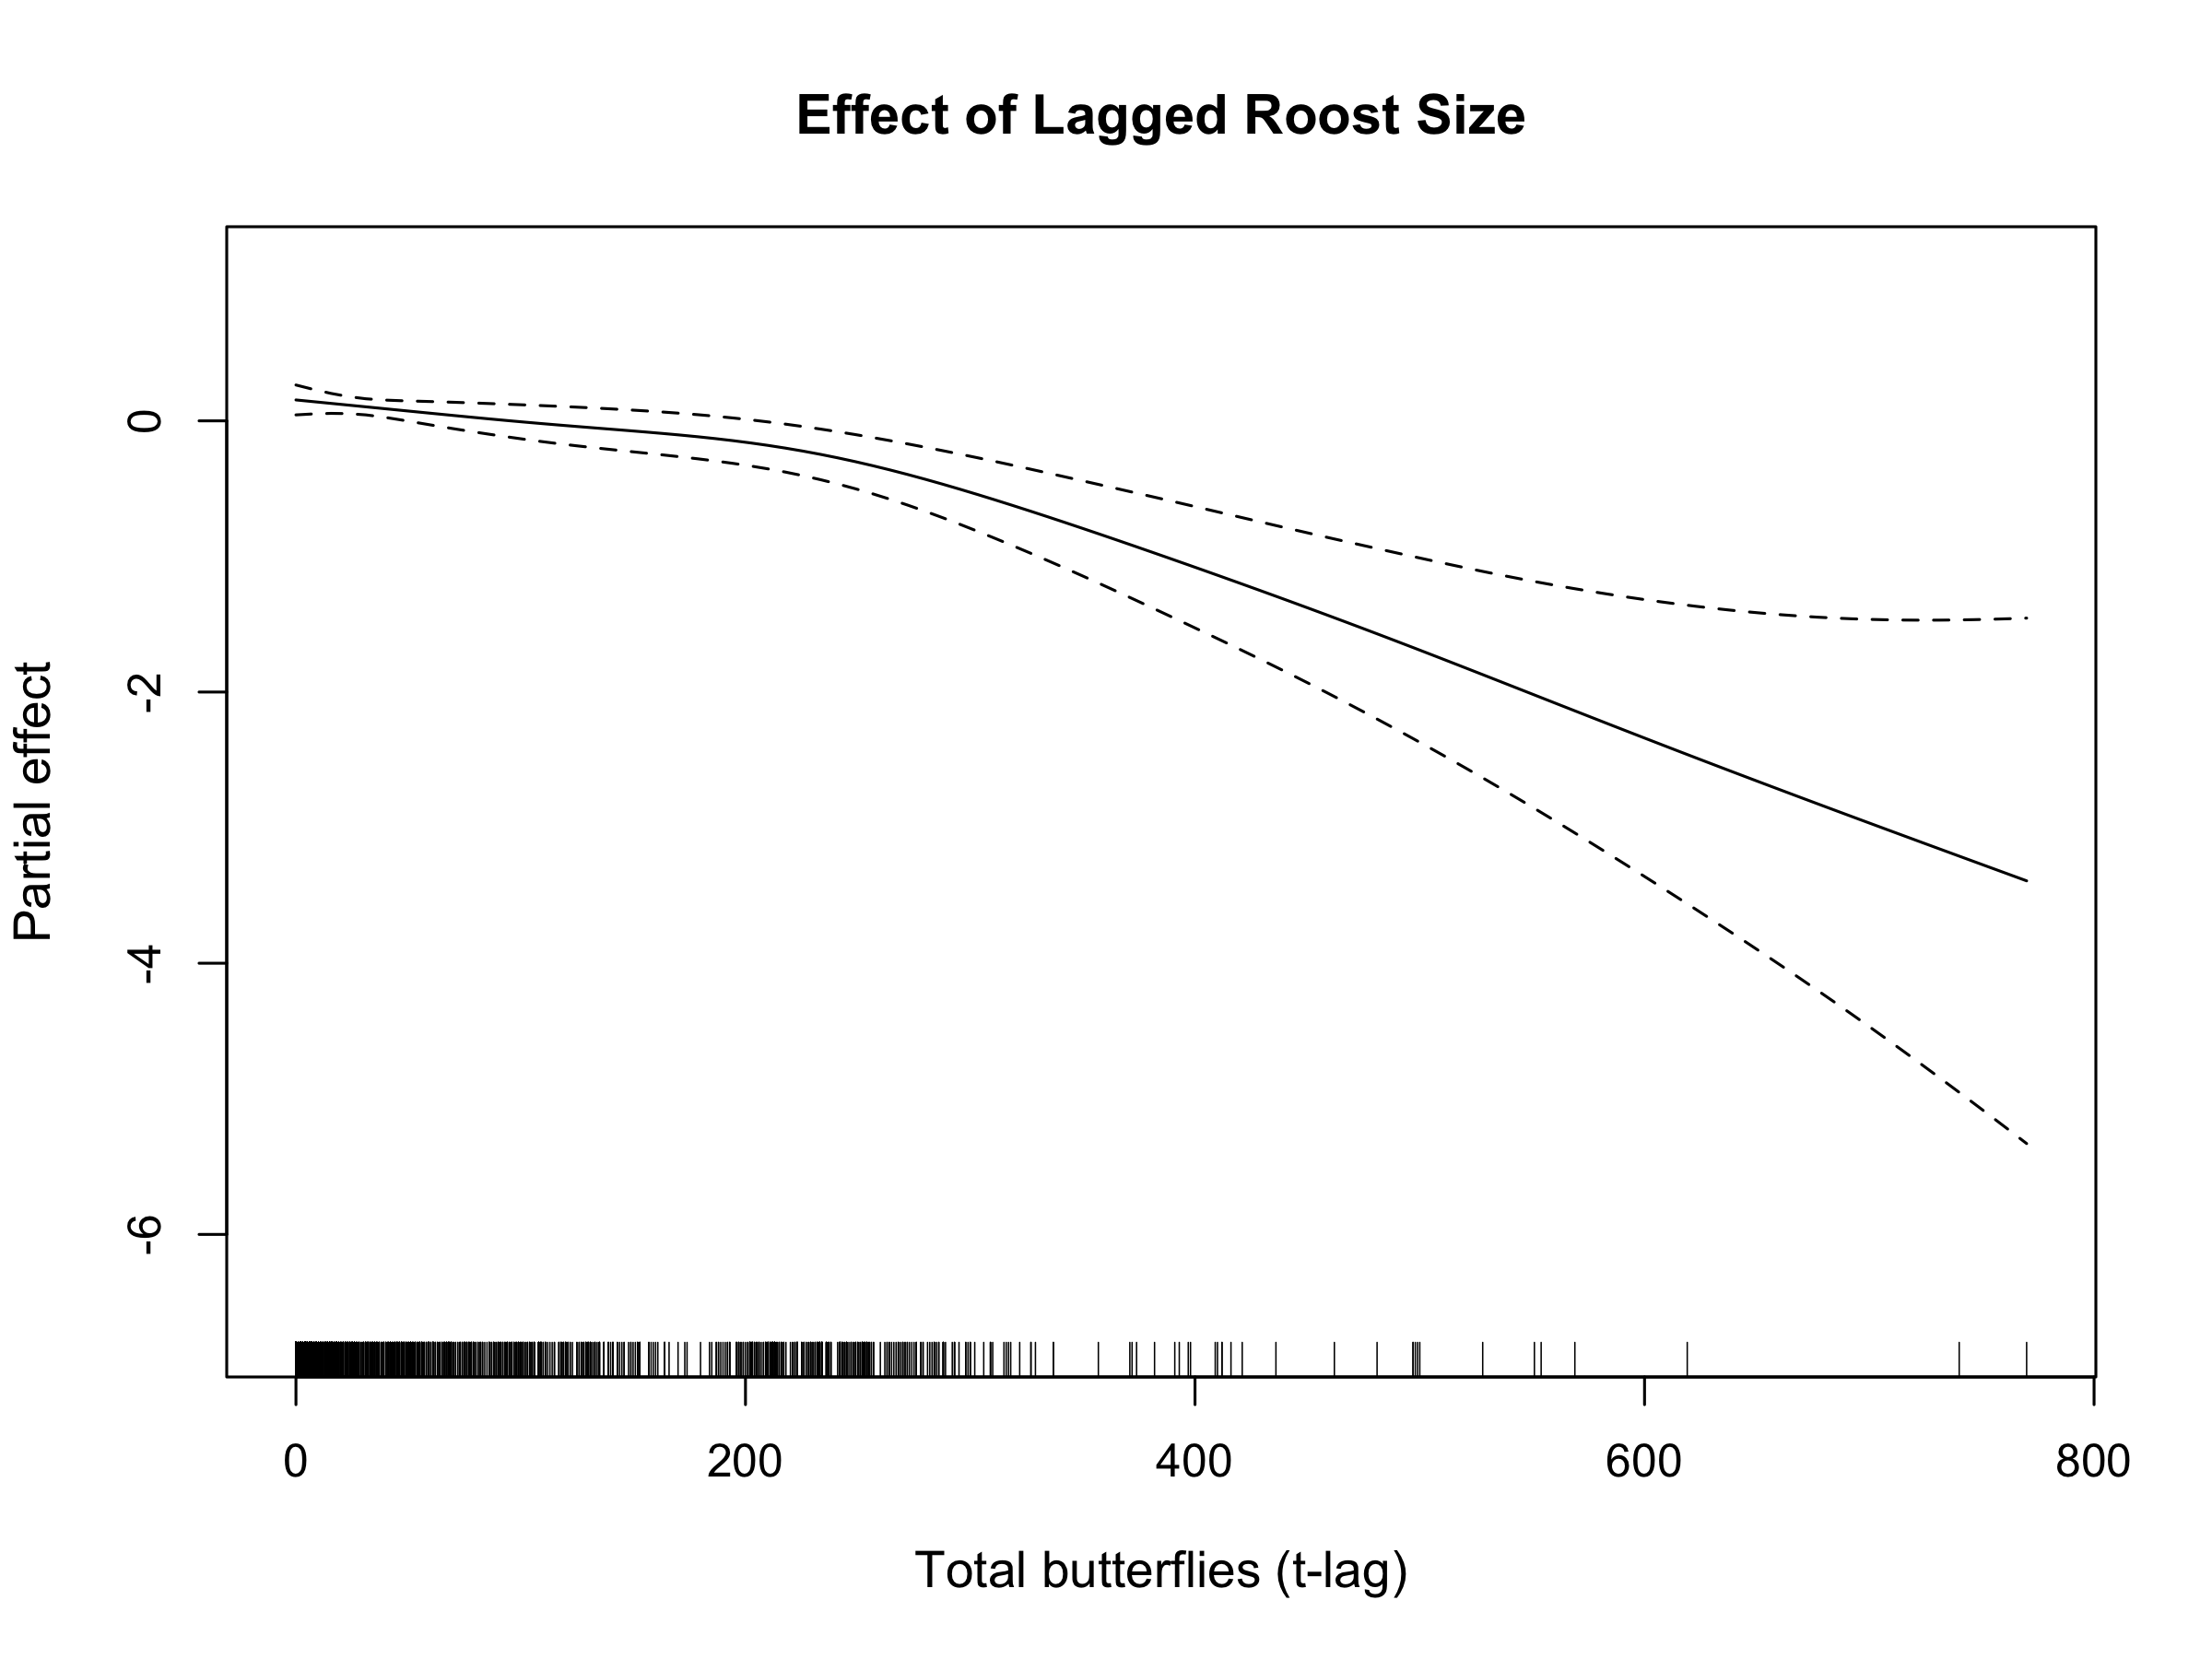
\includegraphics[width=0.8\textwidth]{supplemental/results/thesis_exports/figures/effect_lagged_roost_size.png}
\caption{Partial effect of previous butterfly count on the cube-root transformed change in abundance. The smooth relationship shows increasing negative changes (more butterflies leaving) as initial roost size increases. Shaded area represents 95\% confidence interval.}
\label{fig:effect_roost_size}
\end{figure}

\begin{figure}[htbp]
\centering
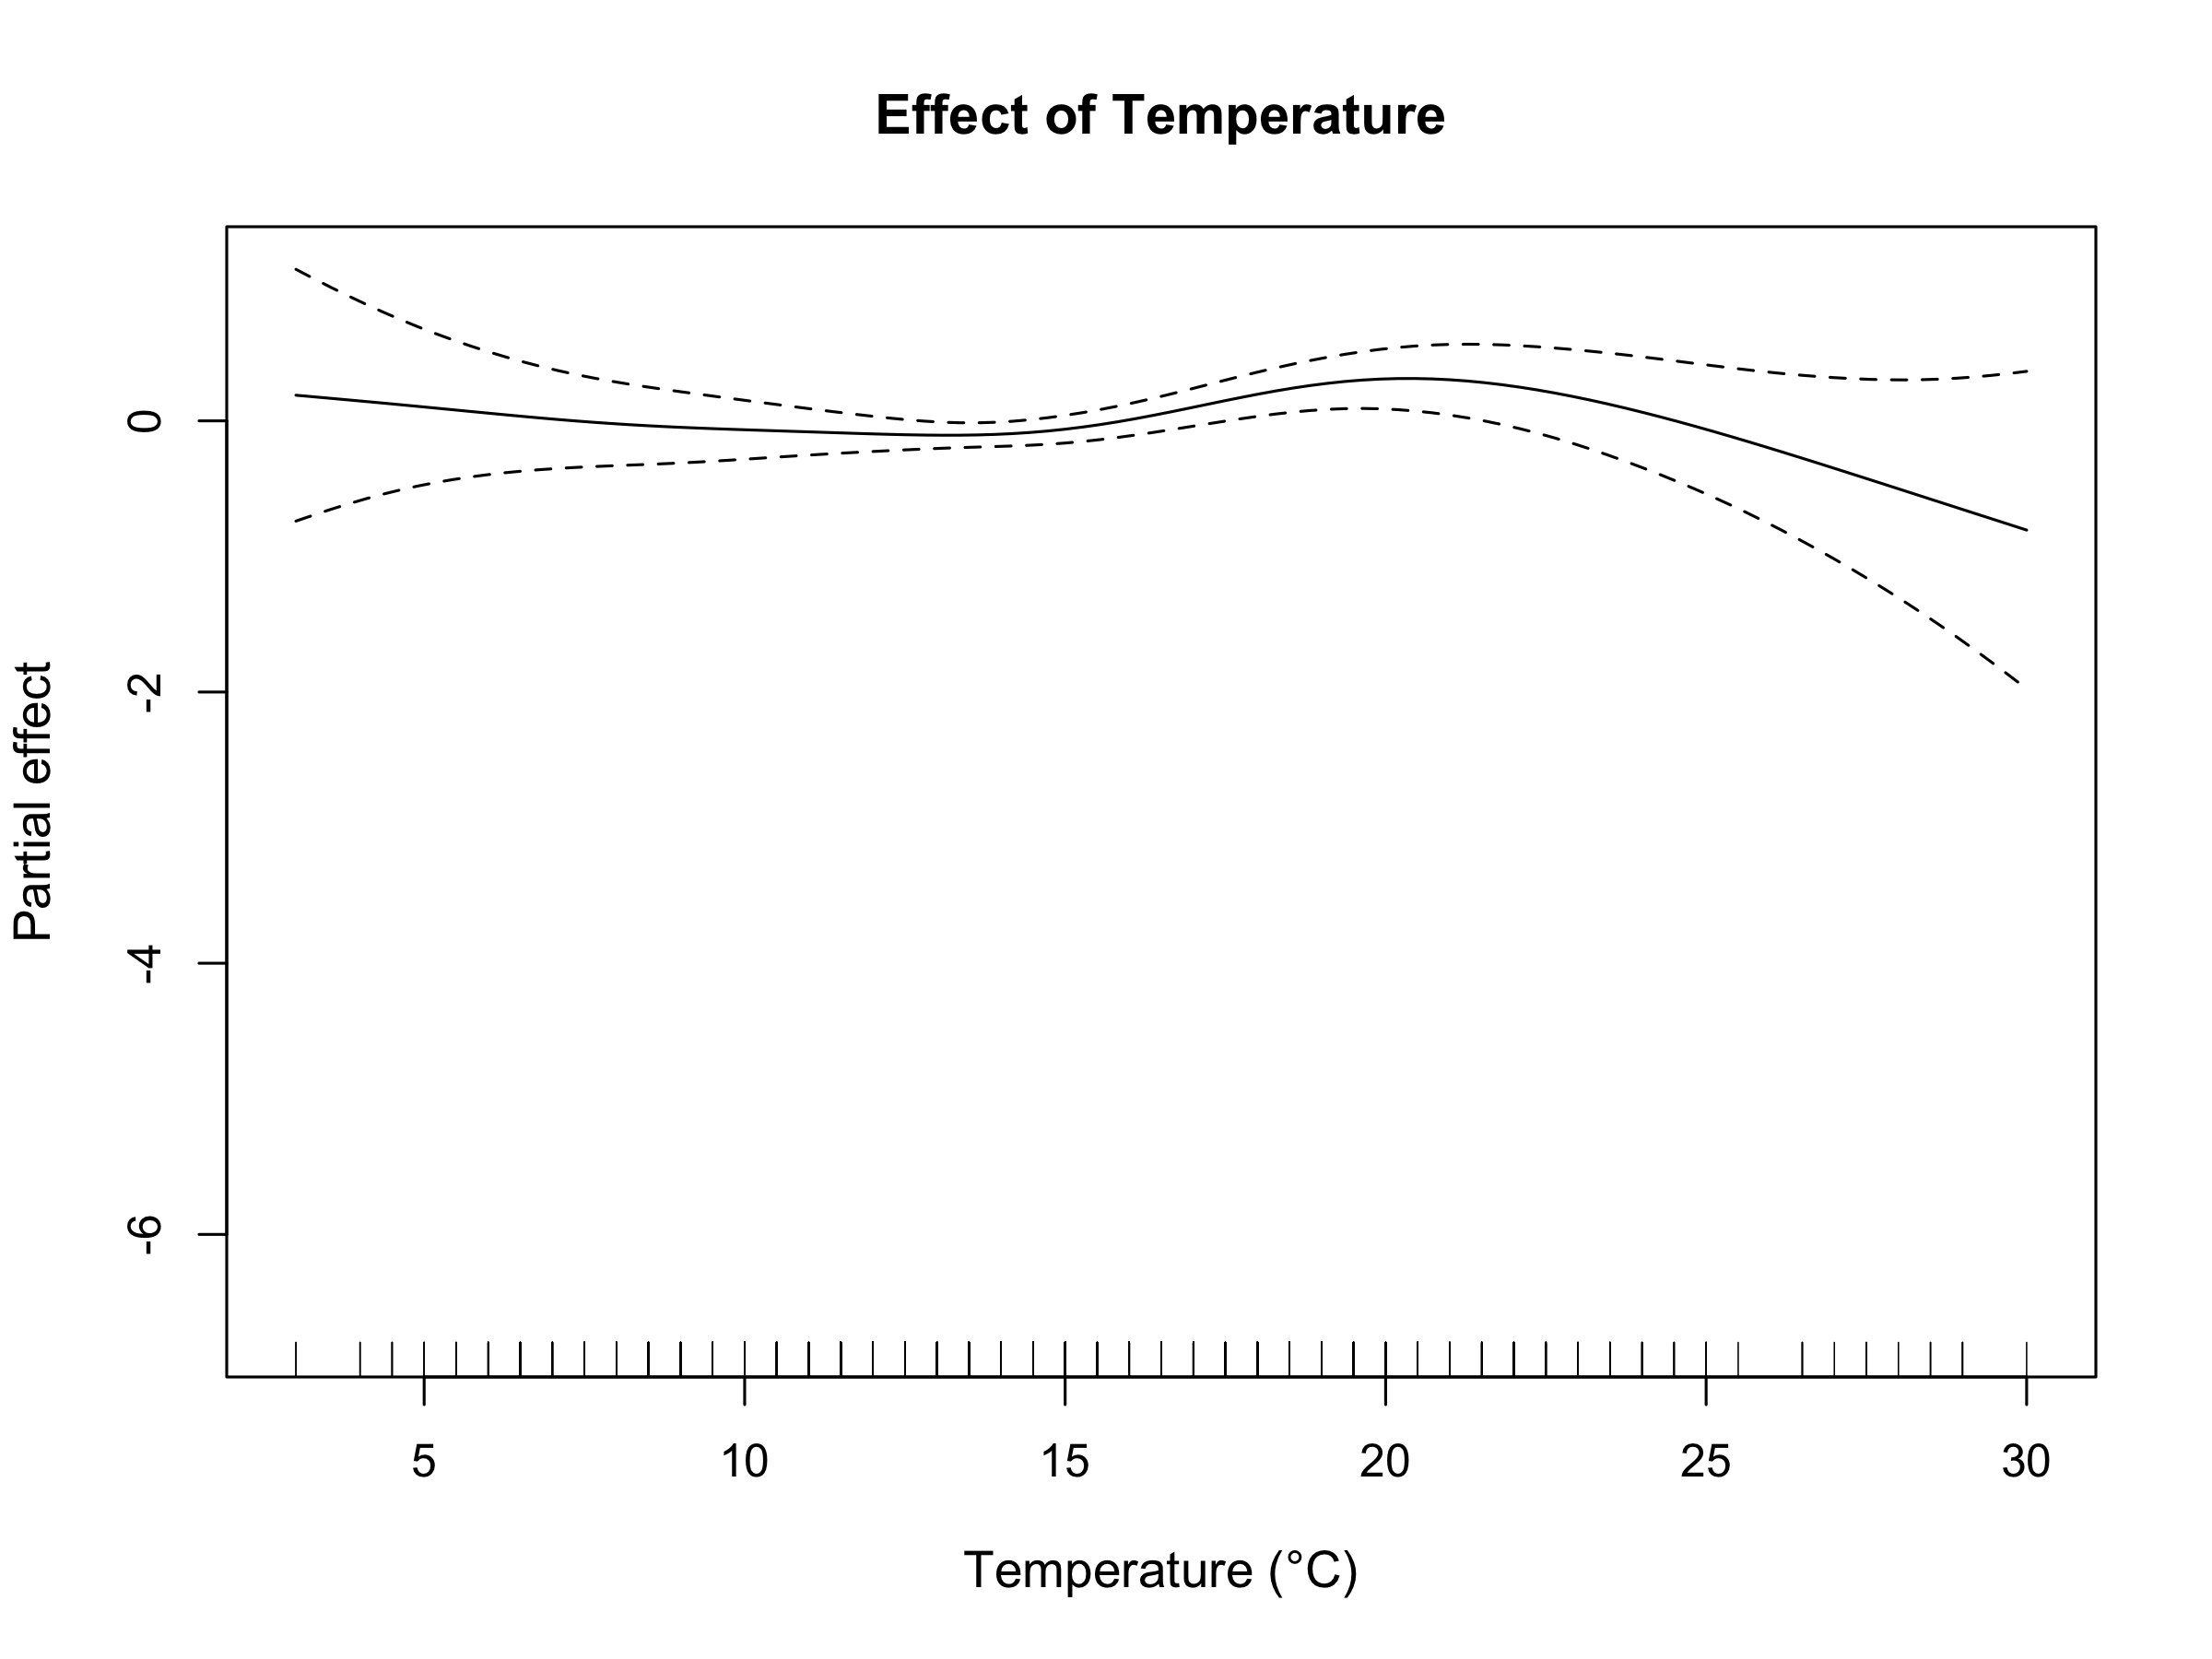
\includegraphics[width=0.8\textwidth]{supplemental/results/thesis_exports/figures/effect_temperature.png}
\caption{Partial effect of average temperature on monarch abundance change. The non-linear relationship peaks at approximately 20°C, suggesting optimal temperatures for monarch activity. Shaded area represents 95\% confidence interval.}
\label{fig:effect_temperature}
\end{figure}

Butterflies exposed to direct sunlight showed a strong negative effect on roost abundance (EDF = 1.53, F = 19.36, p < 0.001), with greater sun exposure associated with larger decreases in total abundance (Figure \ref{fig:effect_sun}). This nearly linear relationship (EDF close to 1) suggests a consistent departure response to solar radiation. Time within day revealed a pronounced diurnal pattern (EDF = 4.90, F = 8.90, p < 0.001), capturing cyclical changes in monarch activity throughout daylight hours (Figure \ref{fig:effect_diurnal}).

\begin{figure}[htbp]
\centering
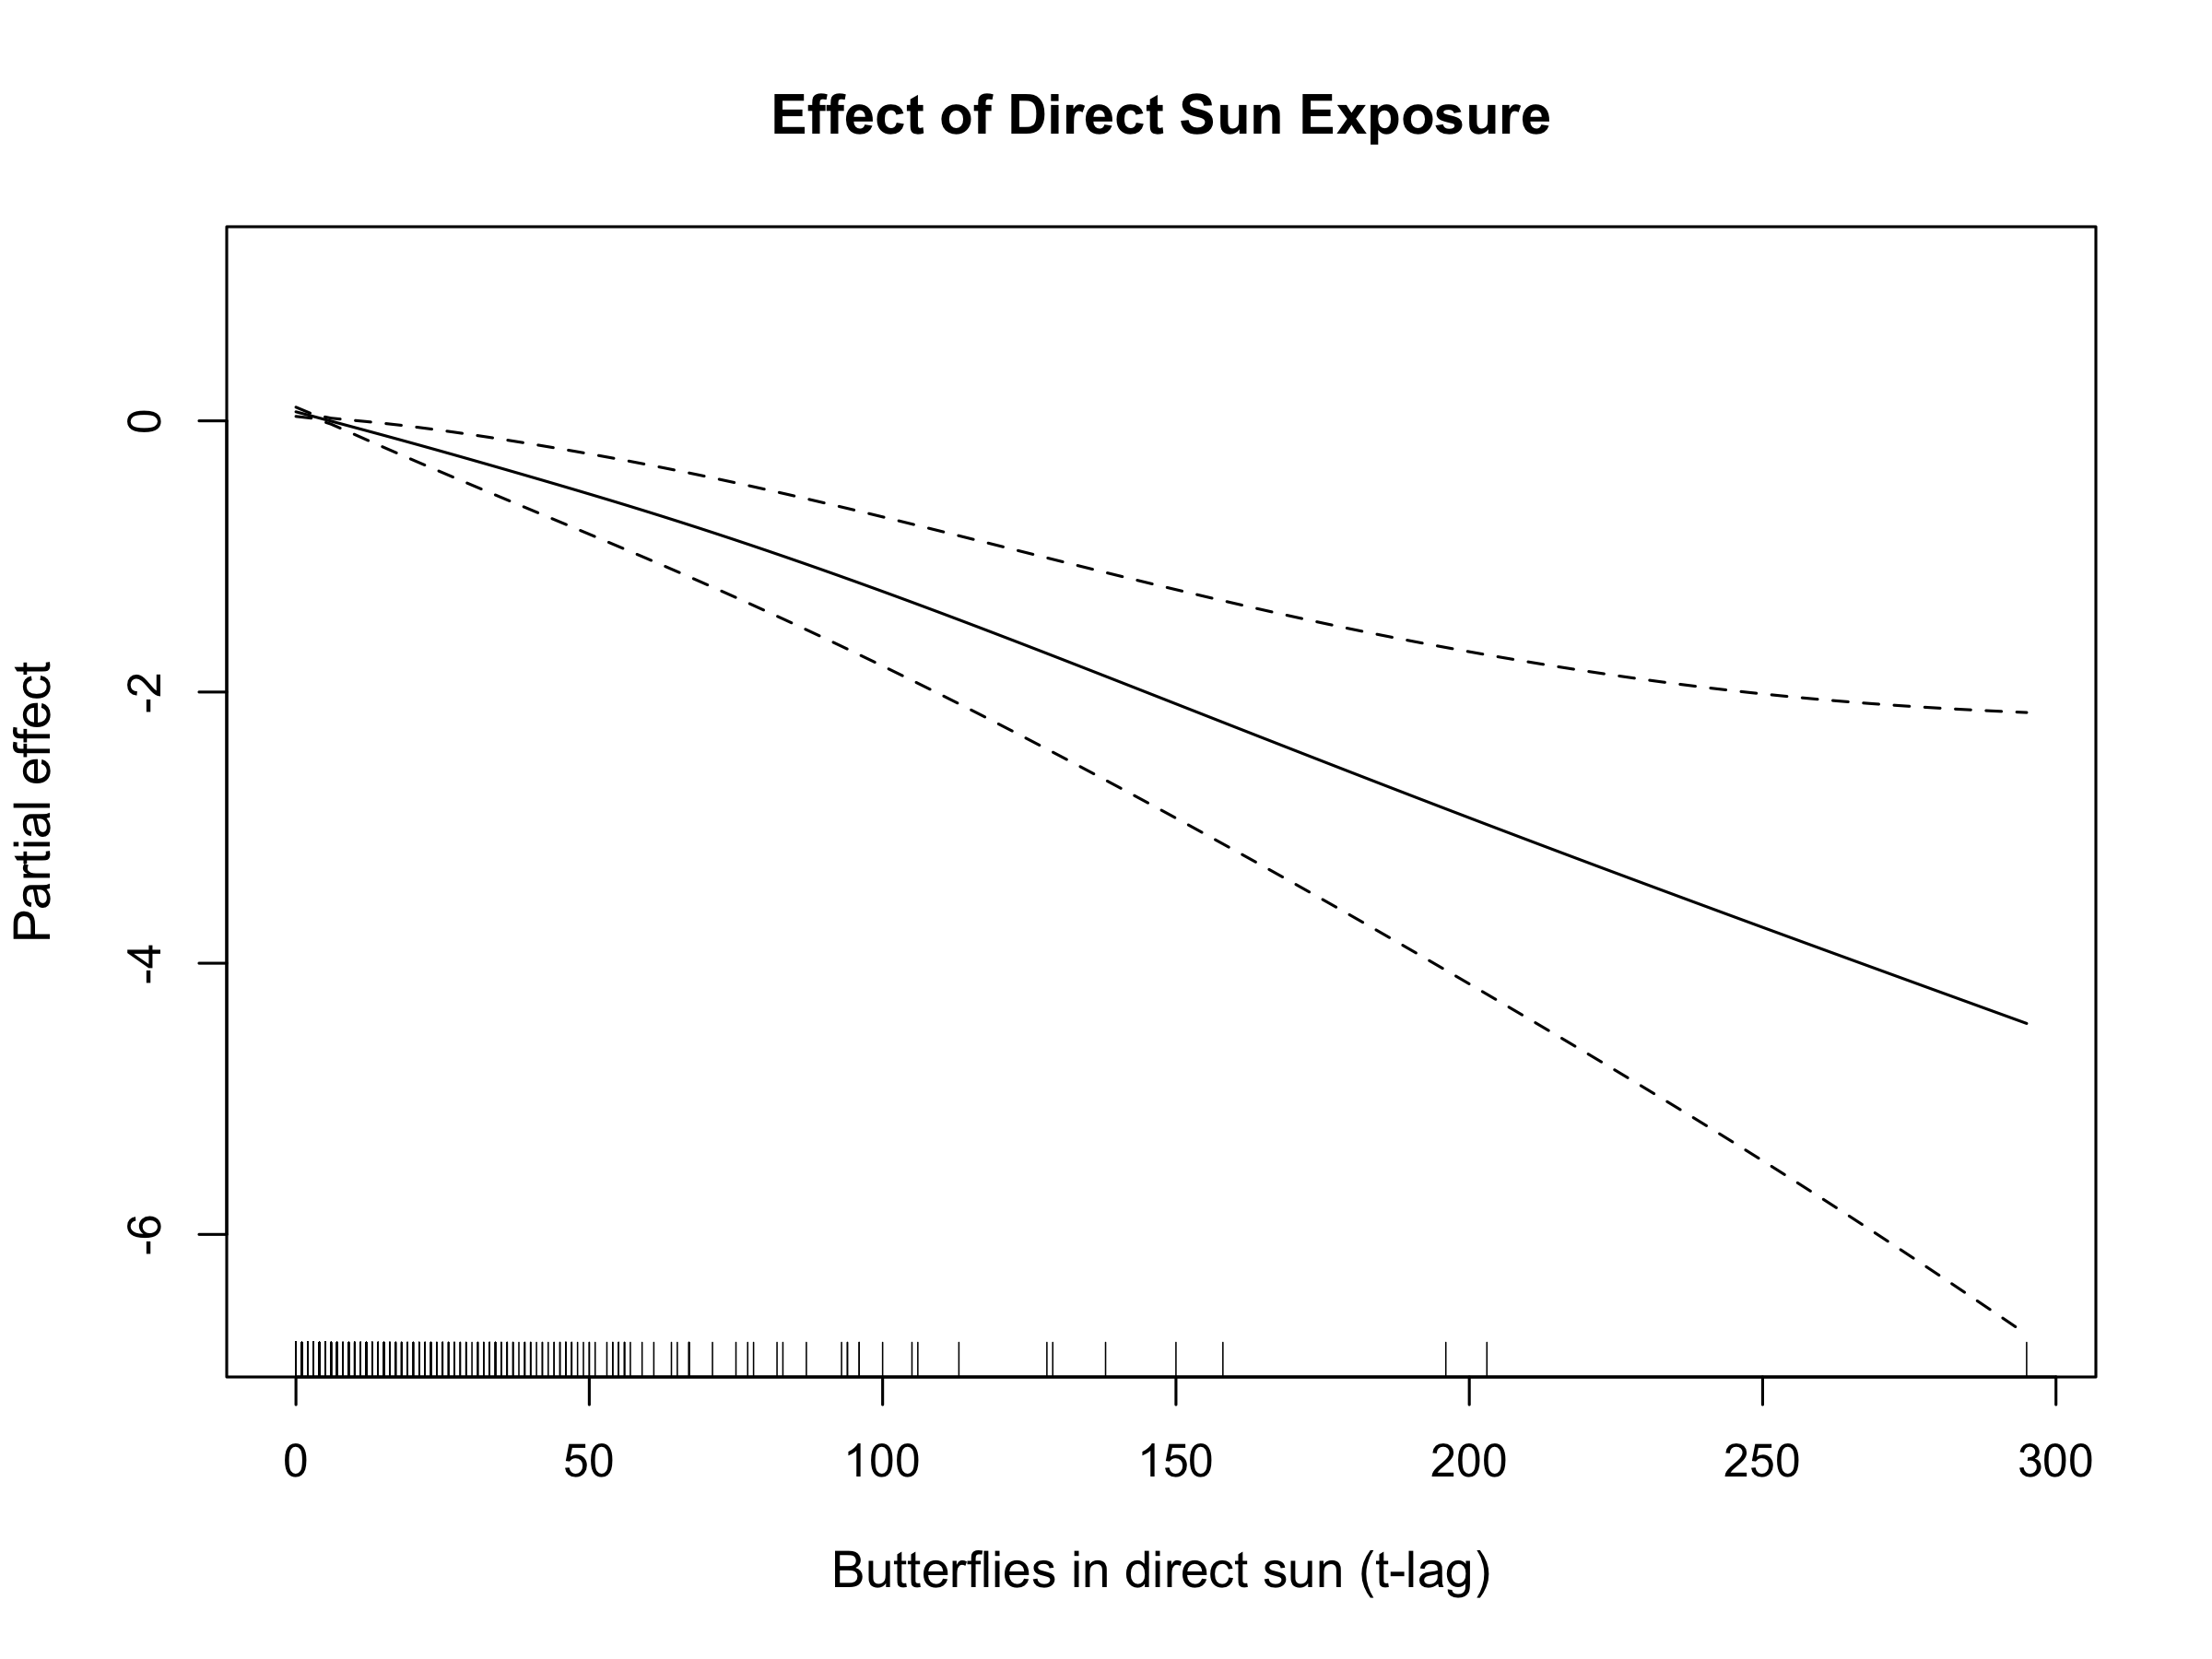
\includegraphics[width=0.8\textwidth]{supplemental/results/thesis_exports/figures/effect_sun_exposure.png}
\caption{Partial effect of butterflies in direct sunlight on abundance change. The negative relationship indicates that greater sun exposure drives departures from the roost. Shaded area represents 95\% confidence interval.}
\label{fig:effect_sun}
\end{figure}

\begin{figure}[htbp]
\centering
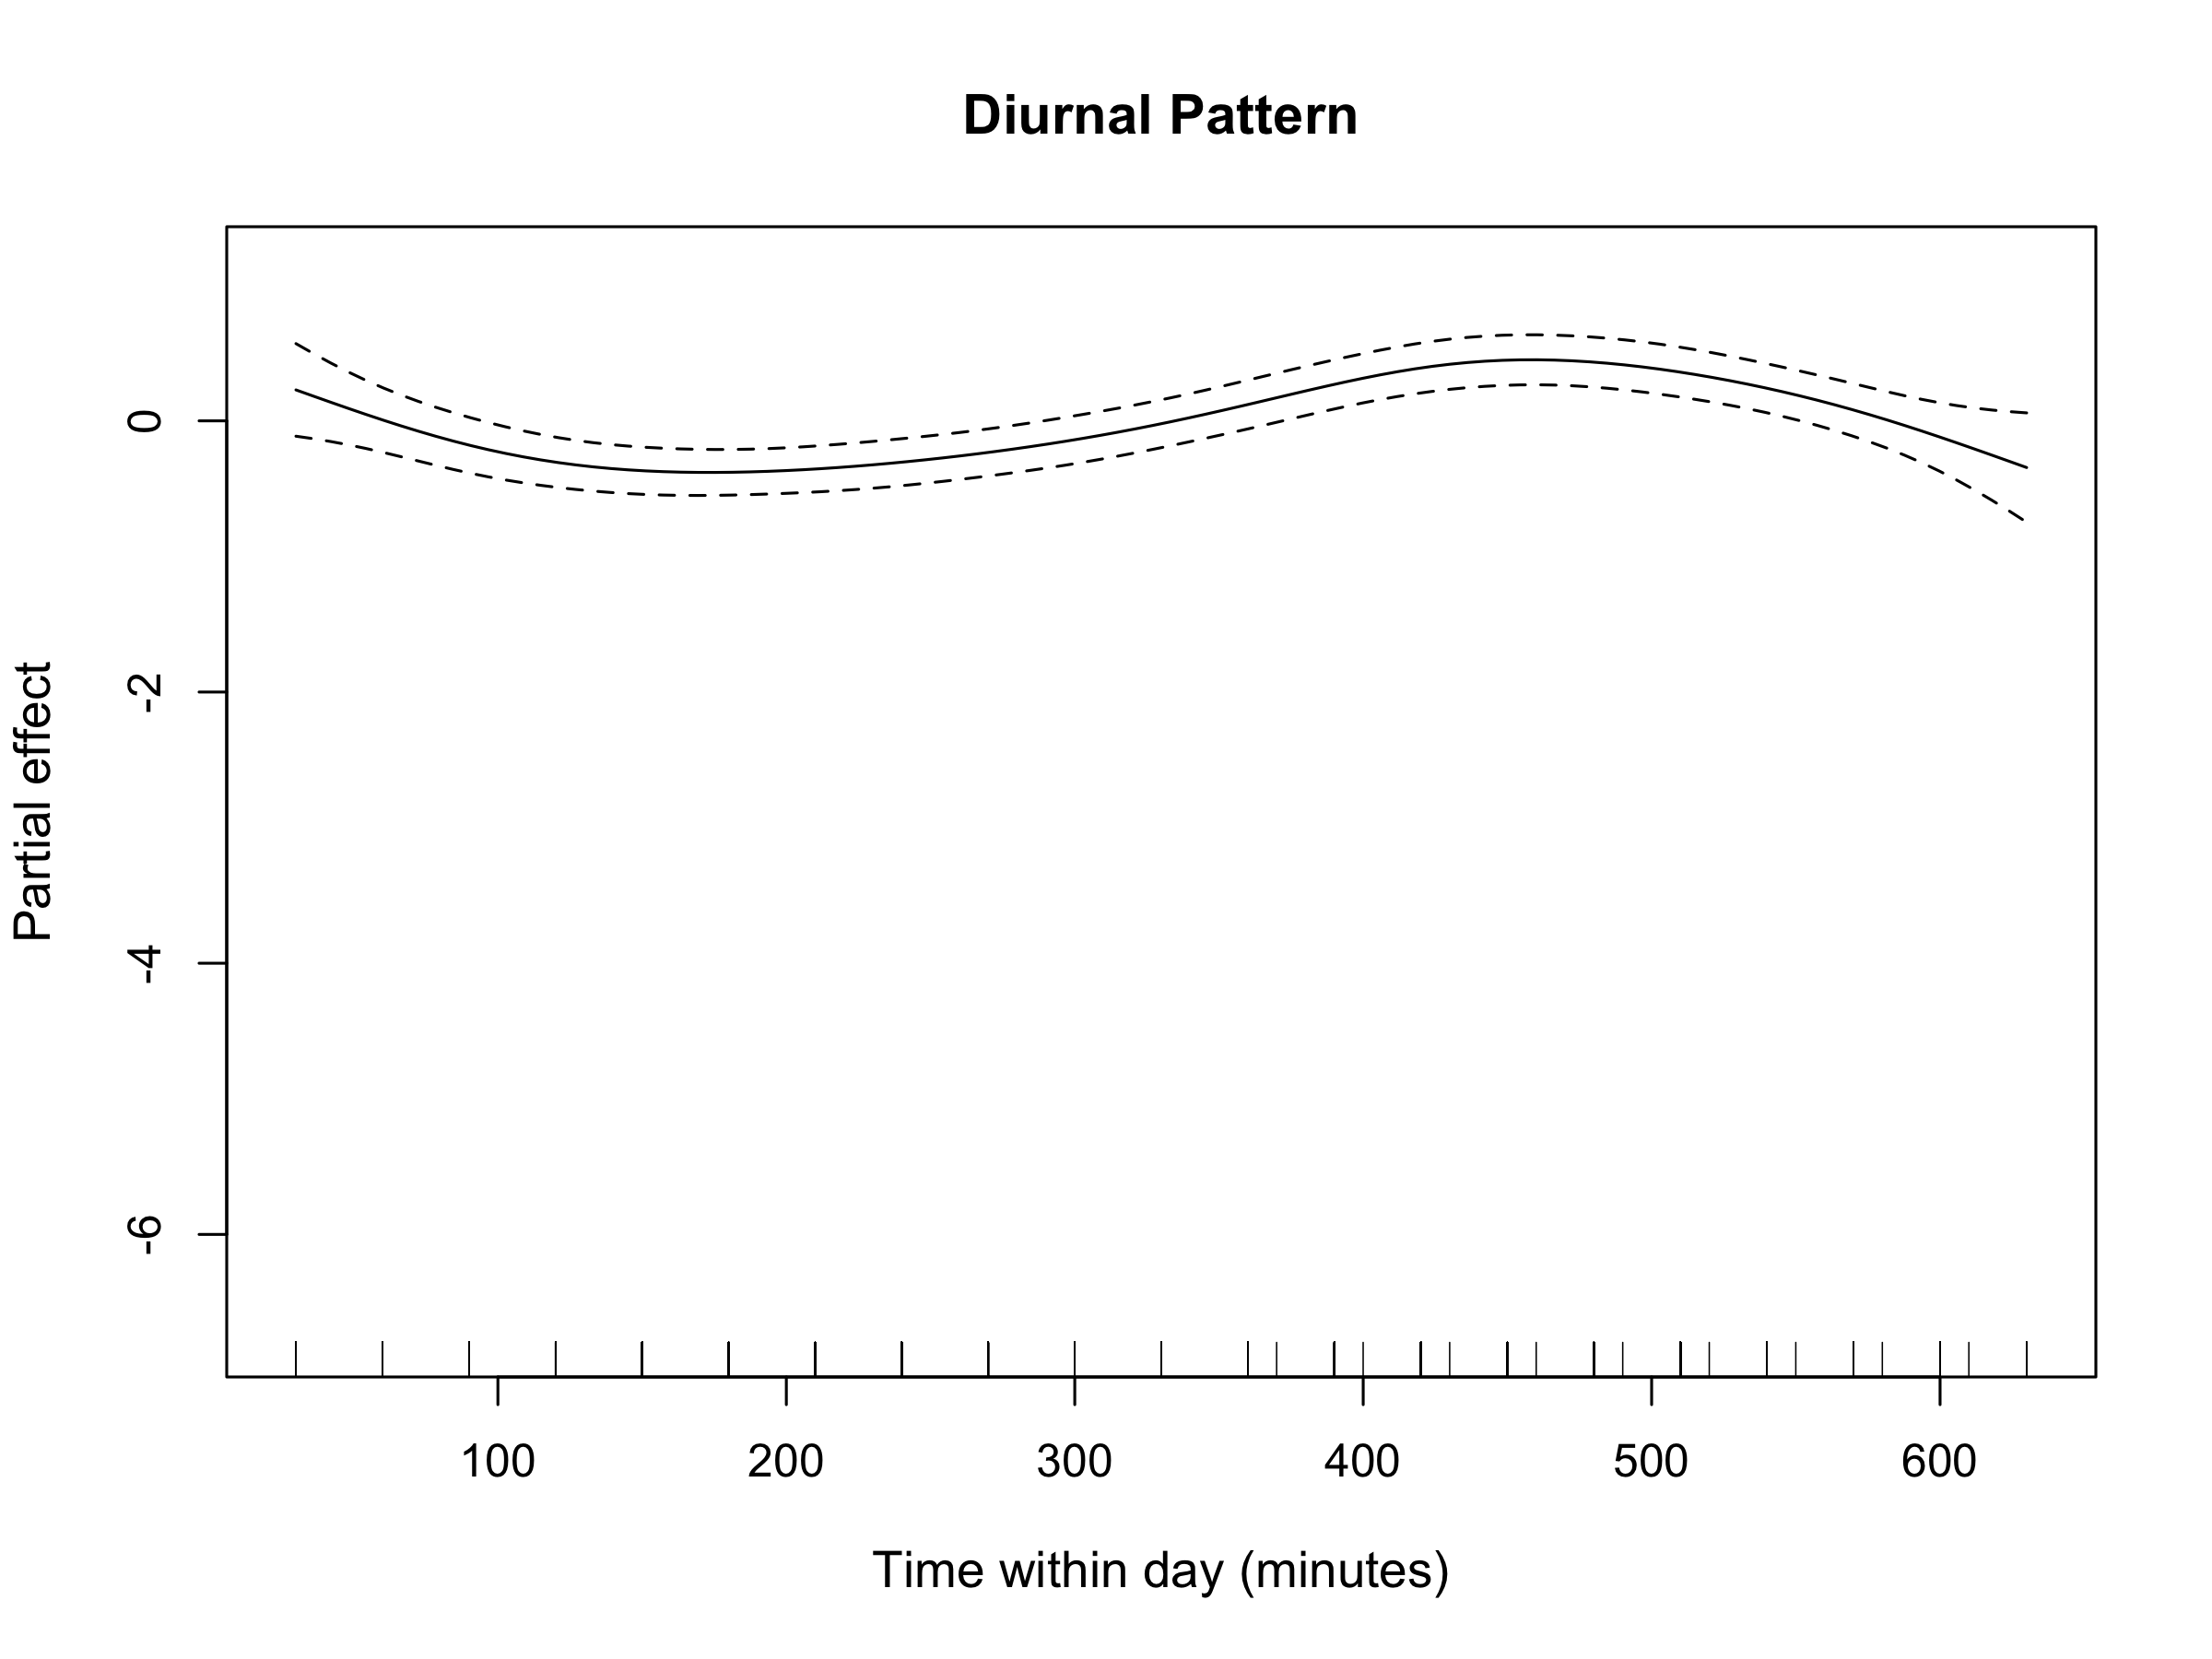
\includegraphics[width=0.8\textwidth]{supplemental/results/thesis_exports/figures/effect_diurnal_pattern.png}
\caption{Diurnal pattern of monarch abundance changes throughout the day. The complex smooth function captures multiple peaks and troughs in activity corresponding to different times of day. Shaded area represents 95\% confidence interval.}
\label{fig:effect_diurnal}
\end{figure}

\subsection{Evaluation of the Disruptive Wind Hypothesis}

Our analysis provided no support for the disruptive wind hypothesis. Wind variables failed to appear in any of the top-performing models, indicating that wind was not a primary driver of monarch abundance changes at overwintering roosts.

The first hypothesis, that wind acts as a disruptive force to overwintering monarchs, was not supported. The AIC-based model selection process did not identify wind as an important predictor, with all top models excluding wind variables entirely. When wind (maximum gust) was forced into the best model structure (M24), model performance declined (\u0394AIC = 6.2), and the wind effect was not statistically significant (p = 0.218).

The second hypothesis, that wind becomes disruptive above a specific 2 m/s threshold, was similarly unsupported. Despite mean wind gusts averaging 2.2 m/s (SD = 1.4 m/s) across our observations—conditions that should have revealed threshold effects if present—we found no evidence for disruption at or above this proposed boundary.

The third hypothesis, that wind's disruptive effects scale with intensity, also lacked support. Maximum gust speed, our measure of wind intensity, showed no relationship with monarch abundance changes. Visual examination confirmed this null relationship, with the scatter plot revealing no trend between wind speed and butterfly departures (Figure \ref{fig:wind_scatter}). The fitted relationship line remained flat across the entire range of observed wind speeds (0–8 m/s), with confidence intervals consistently encompassing zero effect.

\begin{figure}[htbp]
\centering
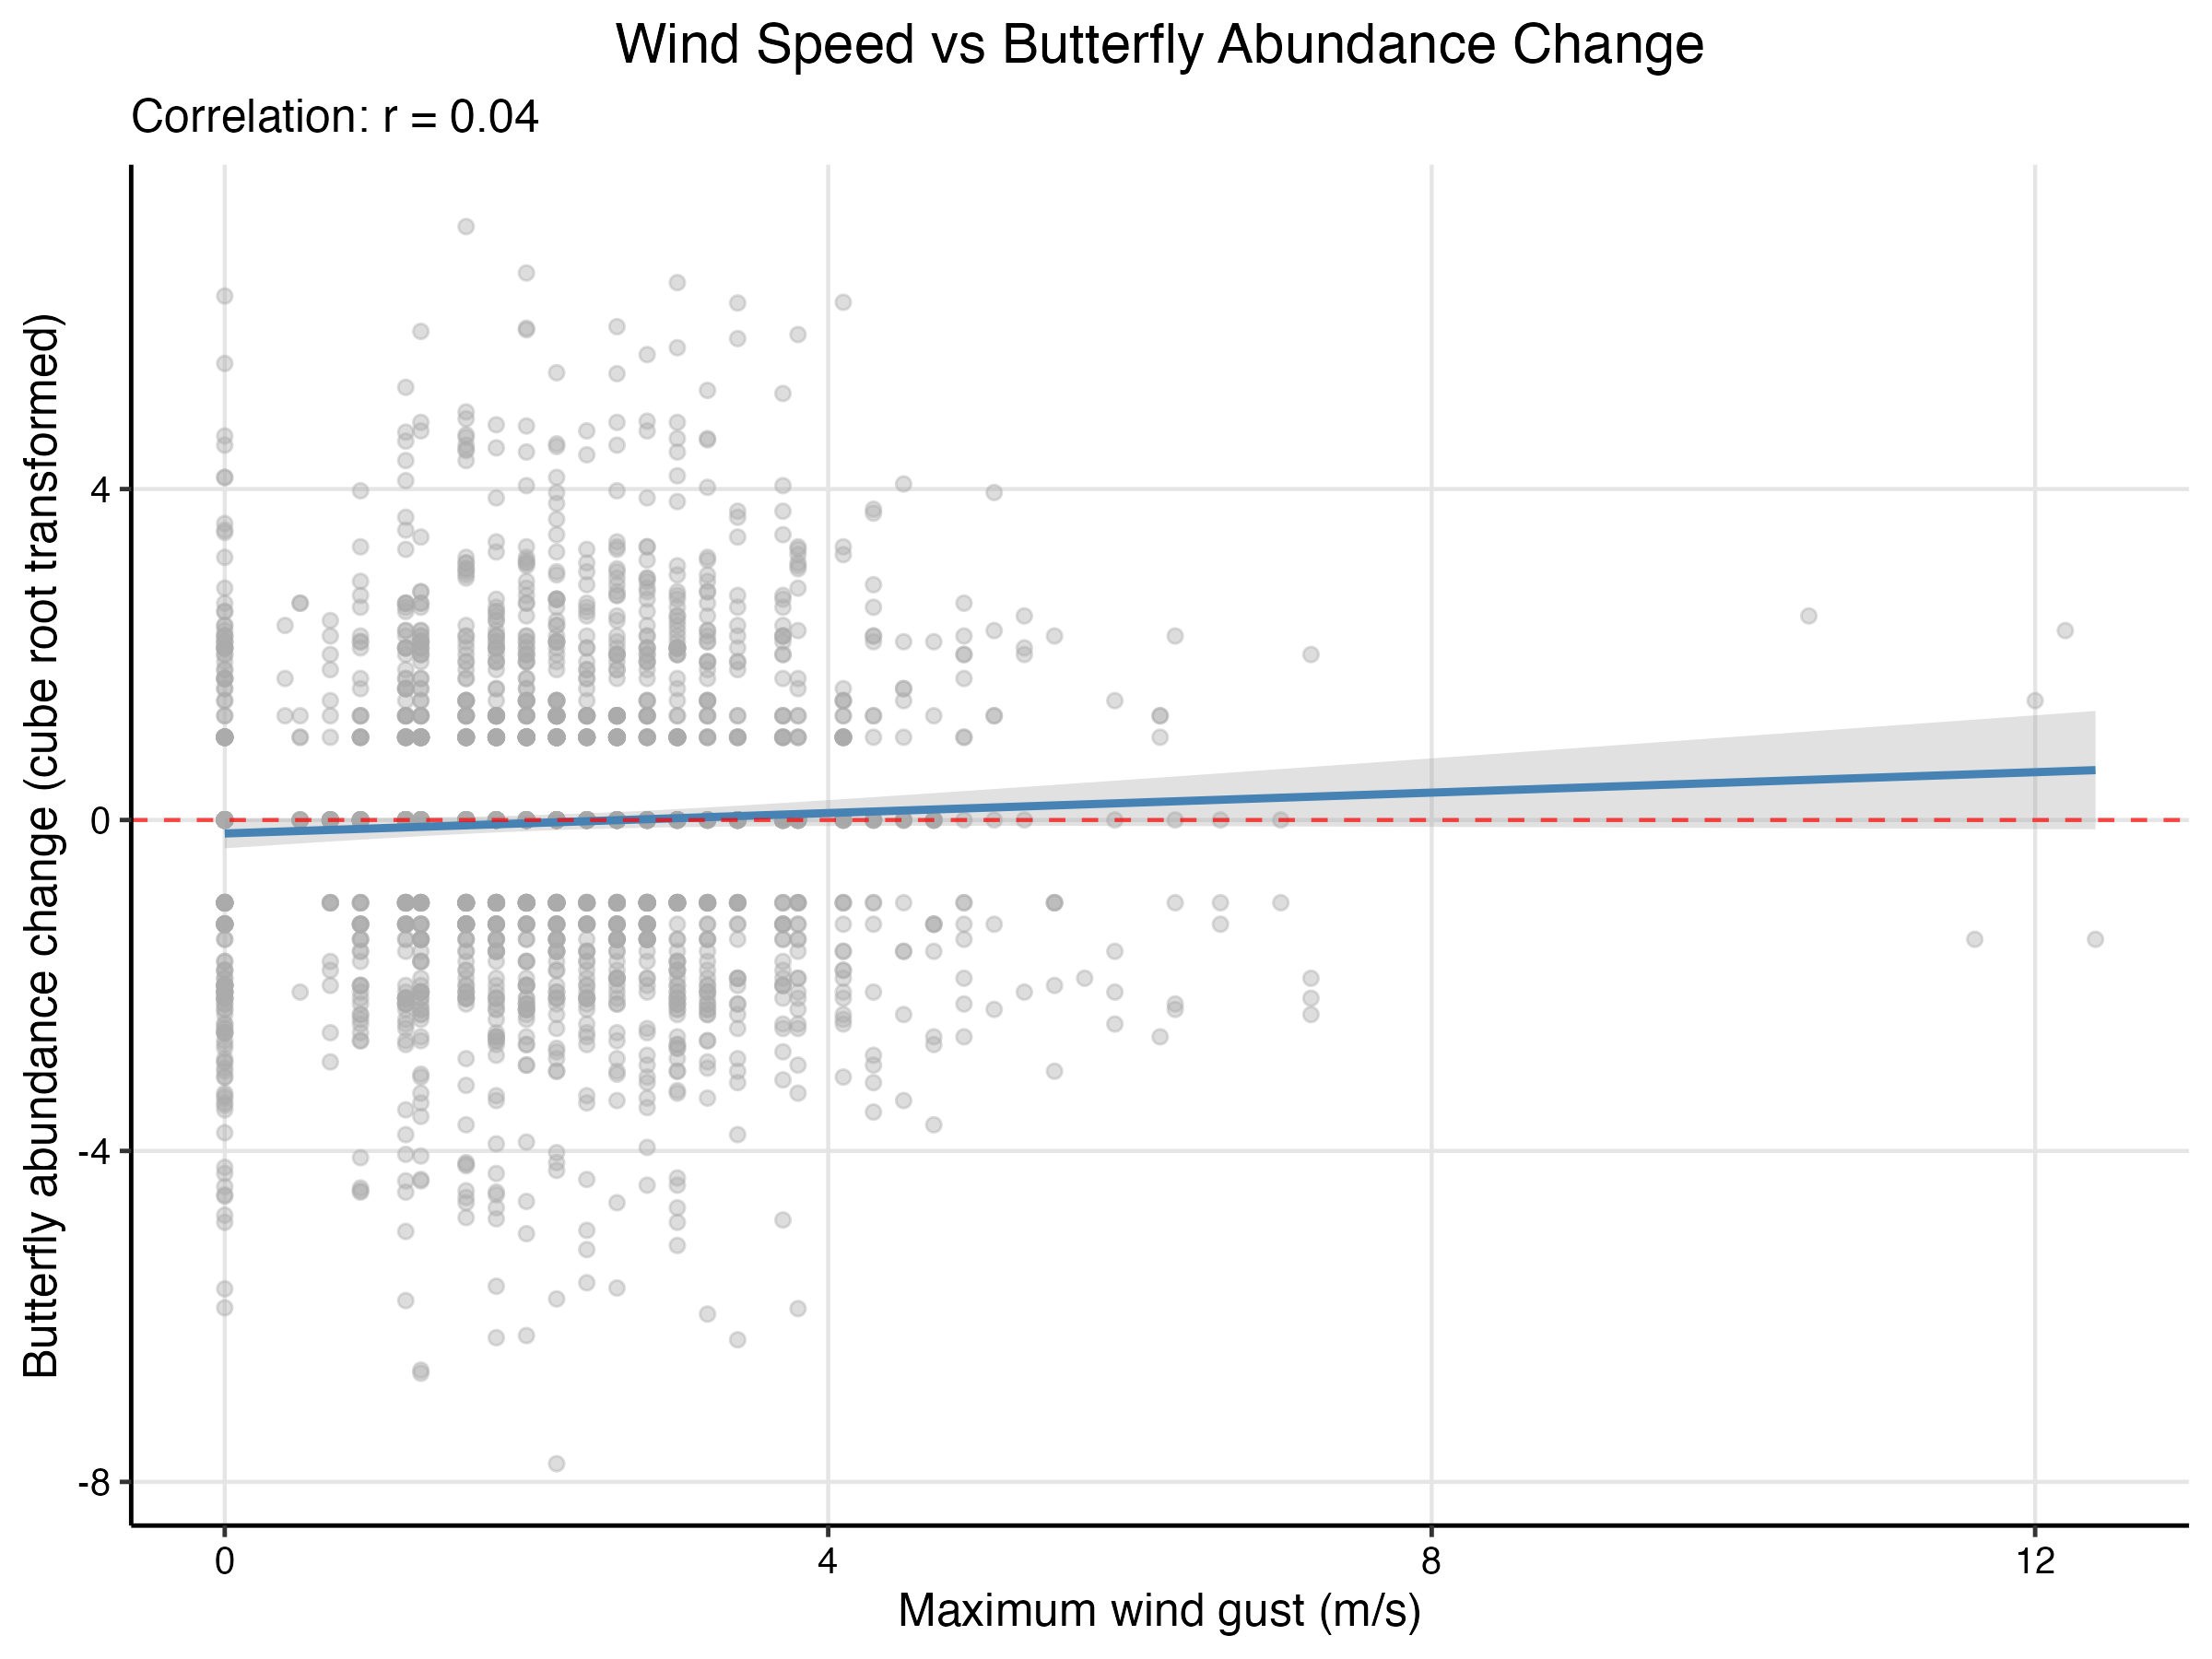
\includegraphics[width=0.8\textwidth]{supplemental/results/thesis_exports/figures/wind_hypothesis_scatter.png}
\caption{Relationship between maximum wind gust speed and cube-root transformed change in monarch abundance. The flat trend line and confidence interval encompassing zero indicate no meaningful relationship between wind speed and butterfly departures from roosts. Points represent individual 30-minute observation periods.}
\label{fig:wind_scatter}
\end{figure}

\subsection{Model Diagnostics}

Examination of model residuals revealed patterns indicative of the discrete nature of our response variable. The residuals versus fitted values plot showed distinct linear banding, an artifact arising from the binned counting method used to estimate butterfly abundance (Figure \ref{fig:residuals}). This patterning, while visually prominent, reflected the methodological constraints of estimating large aggregations rather than model misspecification.

\begin{figure}[htbp]
\centering
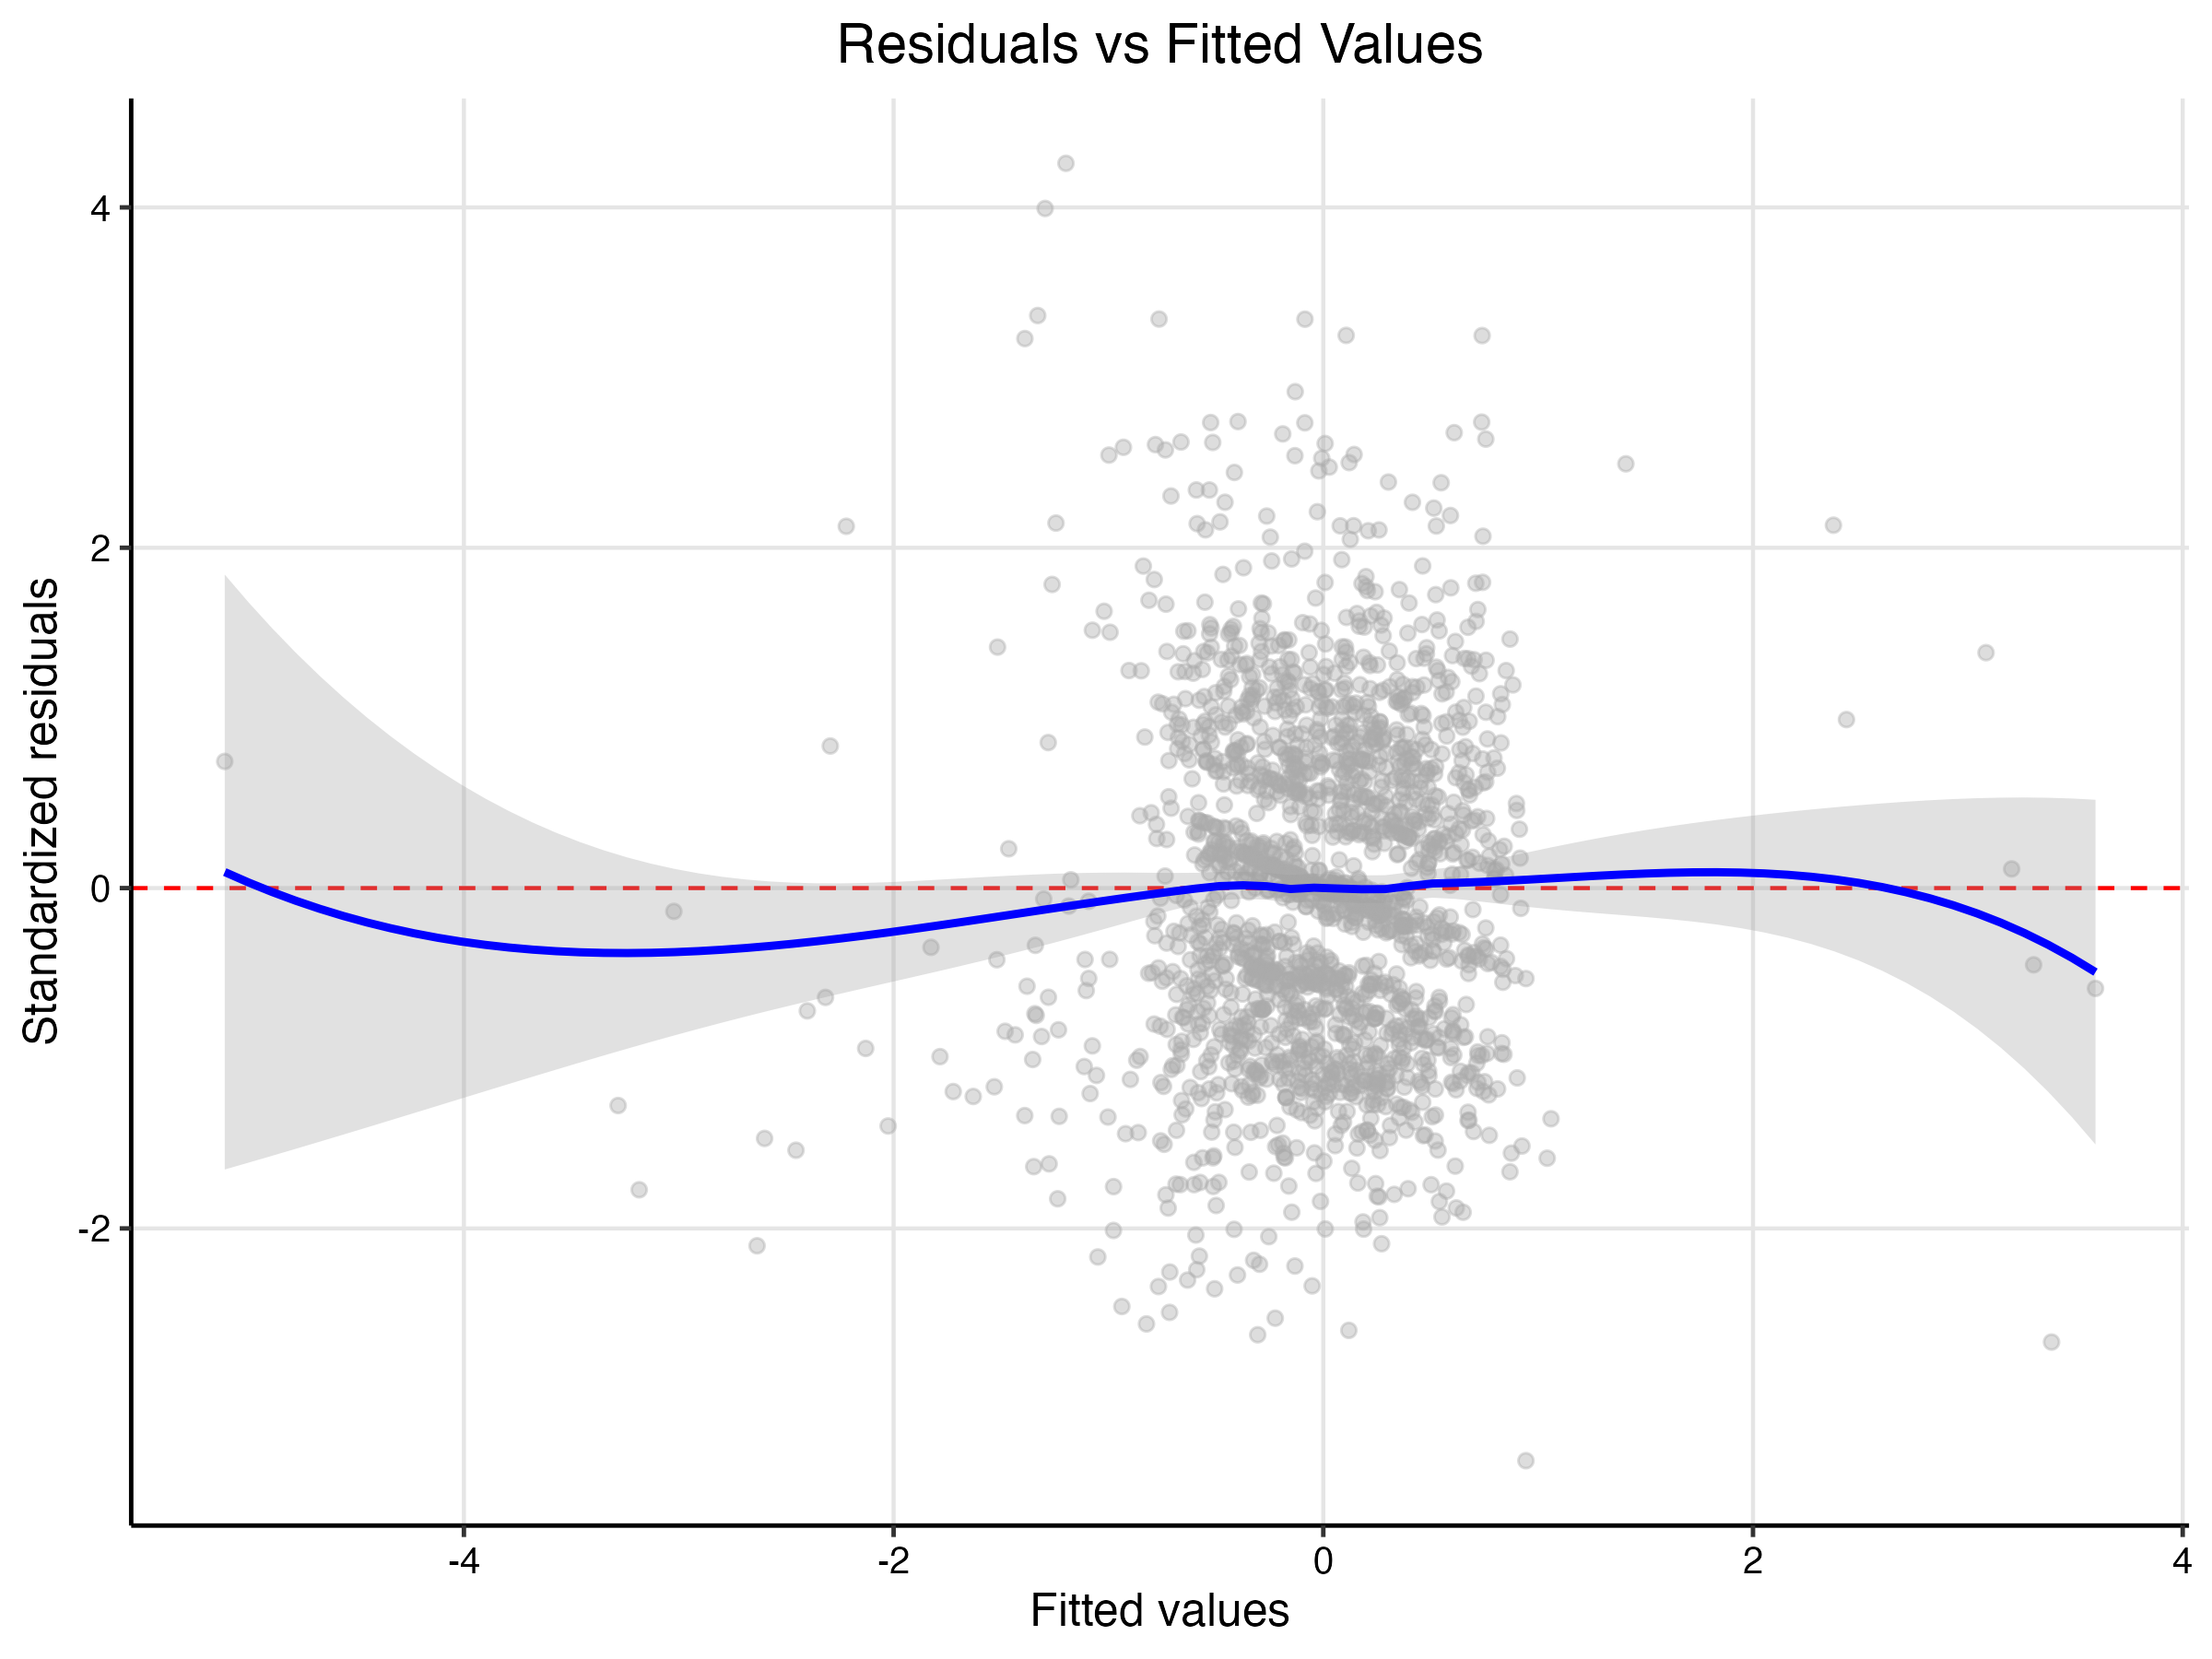
\includegraphics[width=0.8\textwidth]{supplemental/results/thesis_exports/figures/residuals_vs_fitted.png}
\caption{Residuals versus fitted values for the best-fit model (M23). The visible linear banding pattern reflects the discrete nature of the response variable arising from order-of-magnitude counting methods. Red line shows the smoothed relationship.}
\label{fig:residuals}
\end{figure}

The normal quantile-quantile plot indicated that model residuals were approximately normally distributed, though with some deviation in the tails (Figure \ref{fig:qqplot}). These tail deviations were consistent with the discrete patterning observed in the residual plot and did not suggest substantial violation of model assumptions. The central portion of the distribution closely followed the theoretical normal line, supporting the validity of our statistical inferences.

\begin{figure}[htbp]
\centering
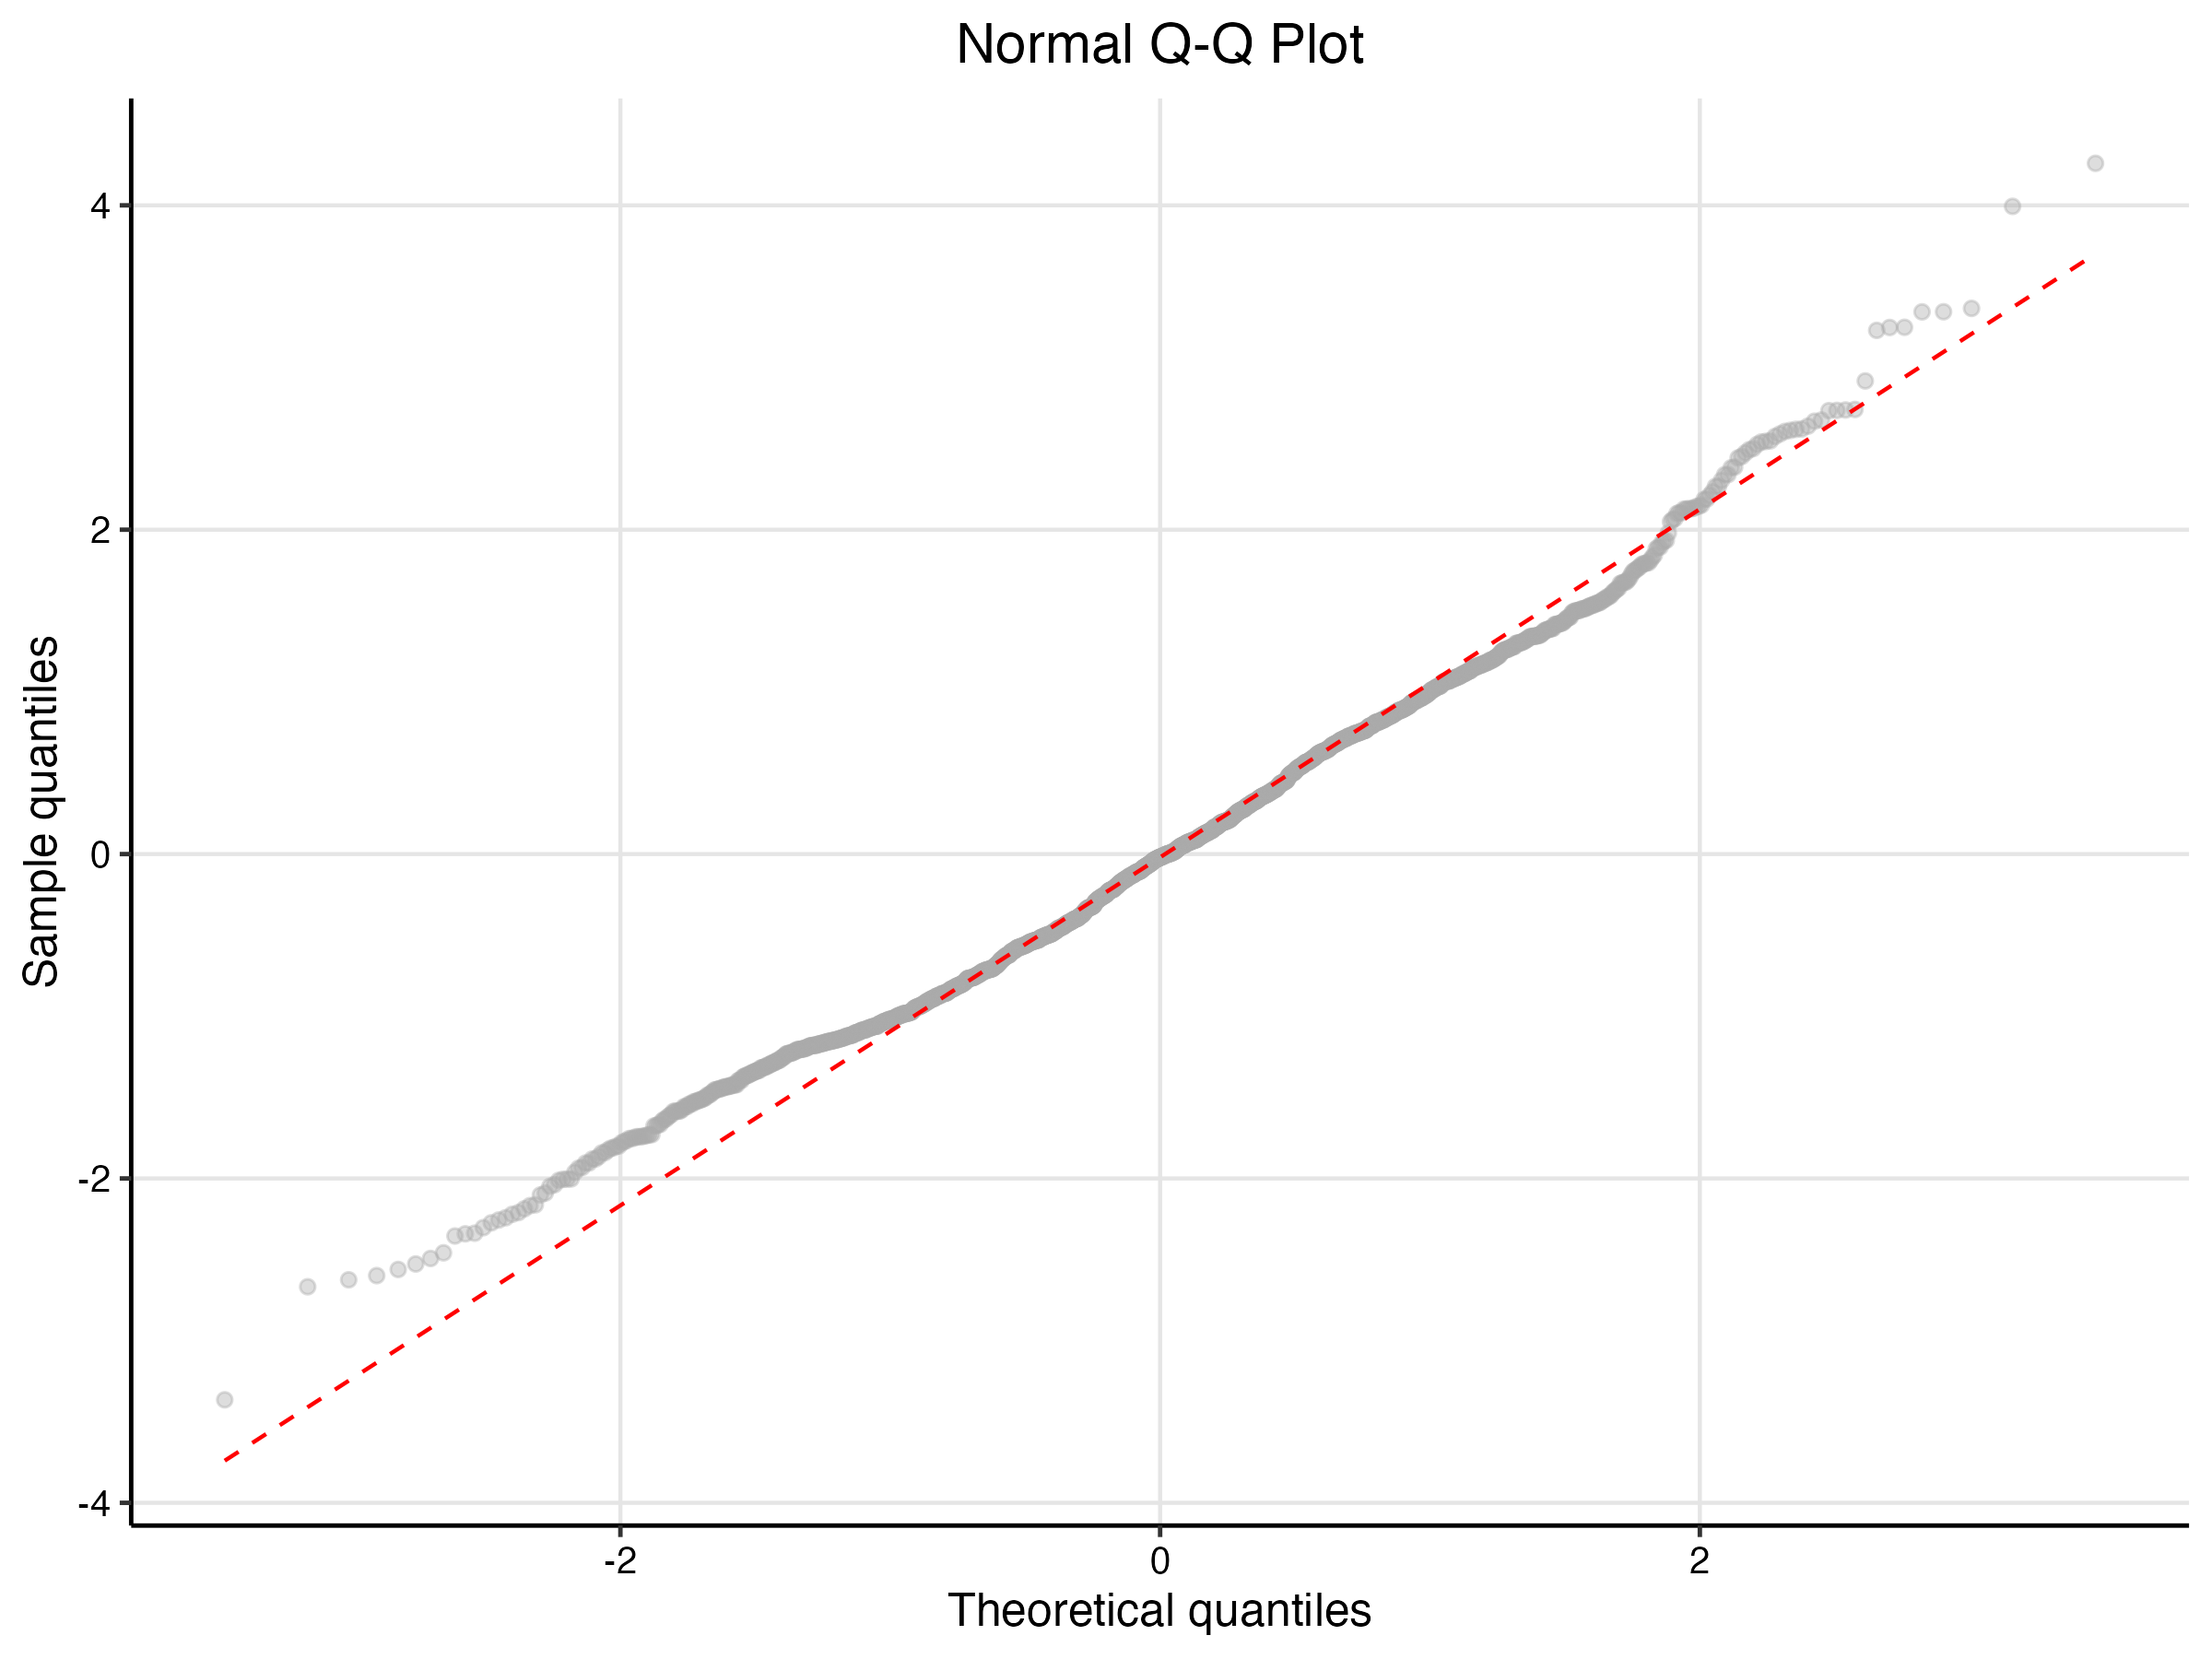
\includegraphics[width=0.8\textwidth]{supplemental/results/thesis_exports/figures/qq_plot.png}
\caption{Normal Q-Q plot of model residuals. The approximately linear relationship indicates reasonable adherence to normality assumptions, with minor deviations in the tails consistent with the discrete nature of the counting method.}
\label{fig:qqplot}
\end{figure}
